\documentclass[tikz]{standalone}
\definecolor{morange}{RGB}{255,127,14}
\definecolor{mblue}{RGB}{31,119,180}
\definecolor{mred}{RGB}{214,39,40}
\definecolor{mpurple}{RGB}{148,103,189}
\definecolor{mgreen}{RGB}{44,160,44}

\newcommand{\pro}{\ensuremath{\mathcal{P}}}
\newcommand{\rec}{\ensuremath{\mathcal{R}}}

\begin{document}
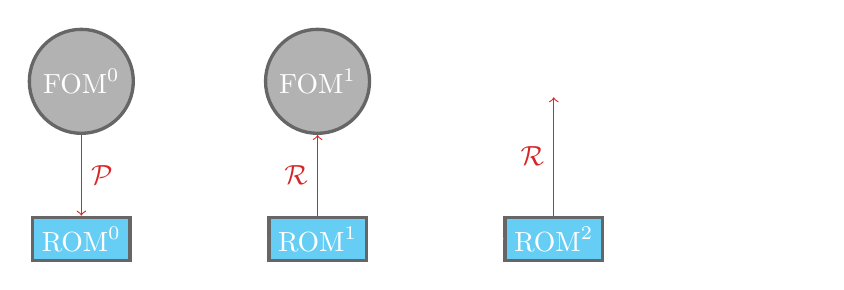
\begin{tikzpicture}[
    squarednodeF/.style={circle, draw=black!60, fill=gray!60, very thick, minimum size=10mm},
    squarednodeR/.style={rectangle, draw=black!60, fill=cyan!60, very thick, minimum size=5mm},
    color = white
    ]
    %Nodes
    \node[squarednodeF]      (full0)                              {$\mathrm{FOM}^0$};
    \node[squarednodeR]        (reduced0)       [below of=full0, yshift=-1cm] {$\mathrm{ROM}^0$};
    \node[squarednodeR]      (reduced1)       [right of=reduced0, xshift=2cm] {$\mathrm{ROM}^1$};
    \node[squarednodeF]        (full1)       [above of=reduced1, yshift=1cm] {$\mathrm{FOM}^1$};
    \node[squarednodeR] (reduced2) [right of=reduced1, xshift=2cm] {$\mathrm{ROM}^2$};
    \node (reduced3) [right of=reduced2, xshift=2cm] {$\cdots$};
    \node (full2) [above of=reduced2, yshift=1cm] {$\cdots$};
    
    %Lines
    \draw[->, mred] (full0.south) to node[right] {\pro} (reduced0.north);
    \draw[->] (reduced0.east) to node[above] {$\mathcal{NN}$} (reduced1.west);
    \draw[->, mred] (reduced1.north) to node[left] {\rec} (full1.south);
    \draw[->, mred] (reduced2.north) to node[left] {\rec} (full2.south);
    \draw[->] (reduced1.east) to node[above] {$\mathcal{NN}$} (reduced2.west);
    \draw[->] (reduced2.east) to node[above] {$\mathcal{NN}$} (reduced3.west);
    \end{tikzpicture}
\end{document}
